%%%%%%%%%%%%%%%%%%%%%%%%%%%%%%%%%%%%%%%%%%%%%%%%%%%%%%%%%%%%%%%%%%
%%%%%%%%%%%%%%%%%%%%%%%%%%%%%%%%%%%%%%%%%%%%%%%%%%%%%%%%%%%%%%%%%%
%Packages
\documentclass[12pt, a4paper]{article}
\usepackage[ margin = 1in]{geometry}
\usepackage{minted, ,amsfonts,amscd, fancyhdr, color, graphicx, environ}
\usepackage{amsmath,amsthm,comment,amssymb}
\usepackage{float}
%\usepackage{mathrsfs}
\usepackage[math-style=ISO]{unicode-math}
\setmathfont{TeX Gyre Termes Math}
\usepackage{lastpage}
\usepackage[dvipsnames]{xcolor}
\usepackage[framemethod=TikZ]{mdframed}
\usepackage{enumerate}
\usepackage[shortlabels]{enumitem}
%\usepackage{fancyhdr}
%\usepackage{indentfirst}
\usepackage{listings}
%\usepackage{sectsty}
%\usepackage{thmtools}
%\usepackage{shadethm}
\usepackage{hyperref}
\usepackage{setspace}
\usepackage{listings}
%\usepackage{mdframed}
%\usepackage{chessfss}
%\usepackage{array}
\usepackage{multicol}
\usepackage{subcaption}
\usepackage{amsmath}
\usepackage[linesnumbered,ruled,vlined]{algorithm2e}
%\usepackage{xcolor}
\usepackage{biblatex} %Imports biblatex package
\addbibresource{bibliography.bib} %Import the bibliography file


\hypersetup{
    colorlinks=true,
    linkcolor=blue,
    filecolor=magenta,      
    urlcolor=blue,
}
%%%%%%%%%%%%%%%%%%%%%%%%%%%%%%%%%%%%%%%%%%%%%%%%%%%%%%%%%%%%%%%%%%
%%%%%%%%%%%%%%%%%%%%%%%%%%%%%%%%%%%%%%%%%%%%%%%%%%%%%%%%%%%%%%%%%%
%Environment setup
\mdfsetup{skipabove=\topskip,skipbelow=\topskip}
\newrobustcmd\ExampleText{%
An \textit{inhomogeneous linear} differential equation has the form
\begin{align}
L[v ] = f,
\end{align}
where $L$ is a linear differential operator, $v$ is the dependent
variable, and $f$ is a given non−zero function of the independent
variables alone.
}
\mdfdefinestyle{theoremstyle}{%
linecolor=black,linewidth=1pt,%
frametitlerule=true,%
frametitlebackgroundcolor=gray!20,
innertopmargin=\topskip,
}
\mdtheorem[style=theoremstyle]{Problem}{Problem}
\newenvironment{Solution}{\textbf{Solution.}}

\definecolor{codegreen}{rgb}{0,0.6,0}
\definecolor{codegray}{rgb}{0.5,0.5,0.5}
\definecolor{codepurple}{rgb}{0.58,0,0.82}
\definecolor{backcolour}{rgb}{0.95,0.95,0.92}

\lstdefinestyle{mystyle}{
    backgroundcolor=\color{backcolour},   
    commentstyle=\color{codegreen},
    keywordstyle=\color{magenta},
    numberstyle=\tiny\color{codegray},
    stringstyle=\color{codepurple},
    basicstyle=\ttfamily\footnotesize,
    breakatwhitespace=false,         
    breaklines=true,                 
    captionpos=b,                    
    keepspaces=true,                 
    numbers=left,                    
    numbersep=5pt,                  
    showspaces=false,                
    showstringspaces=false,
    showtabs=false,                  
    tabsize=2
}

\lstset{style=mystyle}
%%%%%%%%%%%%%%%%%%%%%%%%%%%%%%%%%%%%%%%%%%%%%%%%%%%%%%%%%%%%%%%%%%
%%%%%%%%%%%%%%%%%%%%%%%%%%%%%%%%%%%%%%%%%%%%%%%%%%%%%%%%%%%%%%%%%%
%Fill in the appropriate information below
\newcommand{\norm}[1]{\left\lVert#1\right\rVert}     
\newcommand\course{CSE 4650}                            % <-- course name   
\newcommand\hwnumber{0}                                 % <-- homework number
\newcommand\Information{Someone}                        % <-- personal information
%%%%%%%%%%%%%%%%%%%%%%%%%%%%%%%%%%%%%%%%%%%%%%%%%%%%%%%%%%%%%%%%%%
%%%%%%%%%%%%%%%%%%%%%%%%%%%%%%%%%%%%%%%%%%%%%%%%%%%%%%%%%%%%%%%%%%
%Page setup
 % \pagestyle{fancy}
% \headheight 35pt
% \lhead{\today}
% \rhead{
\includegraphics[height=1.4cm]{logo iut.png}}
\lfoot{}
\pagenumbering{arabic}
\cfoot{\small\thepage}
\rfoot{}
\headsep 1.2em
\renewcommand{\baselinestretch}{1.25}
%%%%%%%%%%%%%%%%%%%%%%%%%%%%%%%%%%%%%%%%%%%%%%%%%%%%%%%%%%%%%%%%%%
%%%%%%%%%%%%%%%%%%%%%%%%%%%%%%%%%%%%%%%%%%%%%%%%%%%%%%%%%%%%%%%%%%
%Add new commands here
\renewcommand{\labelenumi}{\alph{enumi})}
\newcommand{\Z}{\mathbb Z}
\newcommand{\R}{\mathbb R}
\newcommand{\Q}{\mathbb Q}
\newcommand{\NN}{\mathbb N}
\newcommand{\PP}{\mathbb P}
\DeclareMathOperator{\Mod}{Mod} 
\renewcommand\lstlistingname{Algorithm}
\renewcommand\lstlistlistingname{Algorithms}
\def\lstlistingautorefname{Alg.}
\newtheorem*{theorem}{Theorem}
\newtheorem*{lemma}{Lemma}
\newtheorem{case}{Case}
\newcommand{\assign}{:=}
\newcommand{\infixiff}{\text{ iff }}
\newcommand{\nobracket}{}
\newcommand{\backassign}{=:}
\newcommand{\tmmathbf}[1]{\ensuremath{\boldsymbol{#1}}}
\newcommand{\tmop}[1]{\ensuremath{\operatorname{#1}}}
\newcommand{\tmtextbf}[1]{\text{{\bfseries{#1}}}}
\newcommand{\tmtextit}[1]{\text{{\itshape{#1}}}}

	
\newcommand{\inlinecode}[1]{{\color{blue}  \texttt{#1}}}

\newenvironment{itemizedot}{\begin{itemize} \renewcommand{\labelitemi}{$\bullet$}\renewcommand{\labelitemii}{$\bullet$}\renewcommand{\labelitemiii}{$\bullet$}\renewcommand{\labelitemiv}{$\bullet$}}{\end{itemize}}
\catcode`\<=\active \def<{
\fontencoding{T1}\selectfont\symbol{60}\fontencoding{\encodingdefault}}
\catcode`\>=\active \def>{
\fontencoding{T1}\selectfont\symbol{62}\fontencoding{\encodingdefault}}
\catcode`\<=\active \def<{
\fontencoding{T1}\selectfont\symbol{60}\fontencoding{\encodingdefault}}

%%%%%%%%%%%%%%%%%%%%%%%%%%%%%%%%%%%%%%%%%%%%%%%%%%%%%%%%%%%%%%%%%%
%%%%%%%%%%%%%%%%%%%%%%%%%%%%%%%%%%%%%%%%%%%%%%%%%%%%%%%%%%%%%%%%%%
%Begin now!

% \setcounter{secnumdepth}{0}

\begin{document}

\begin{titlepage}
    \begin{figure}[!h]
    \centering
    
\includegraphics[width=.2\textwidth]{logo iut.png}
\end{figure}
\begin{center}
\Huge{\textbf{Islamic University of Technology}}\\
\vspace{1.5cm}
\large{CSE 4810}\\
\large{Algorithm Engineering Lab}

\noindent\rule{\textwidth}{1.5pt}
\Large{Lab 0} \\
\noindent\rule{\textwidth}{1.5pt}
\end{center}


\vspace{0.5cm}
\begin{center}
% \begin{multicols}{2}
    \large{
    Name: Tasnimul Hasnat\\
    ID: 190041113\\
    Section 1A\\
    }
% \end{multicols}
 \today
\end{center}

\end{titlepage}


\thispagestyle{empty}
{
  \hypersetup{linkcolor=black}
  \tableofcontents
}


\newpage
\pagenumbering{arabic}
\section{Task 1}
\subsection{Problem}
Sort and draw the following functions with desmos in increasing order of asymptotic (big-O) complexity with justification:
\begin{enumerate}
    \item $f_1(n) = n^{0.999}.\log_2(n)$
    \item $f_2(n) = \binom{n}{2}$
    \item $f_3(n) = (1000001 * 10^{-6})^{n}$
    \item $f_4(n) = n!$
    \item $f_5(n) = 2^{(10*10^{7})}$
    \item $f_6(n) = n*\sqrt{n}$
    \item $f_7(n) = n^{\sqrt{n}}$
    \item $f_8(n) = \sum_{i=1}^{n} (i+1)$    
\end{enumerate}

\subsection{Graph}
Plotting the given functions in desmos graphing calculator we get -
\begin{figure}[h]
    \centering
    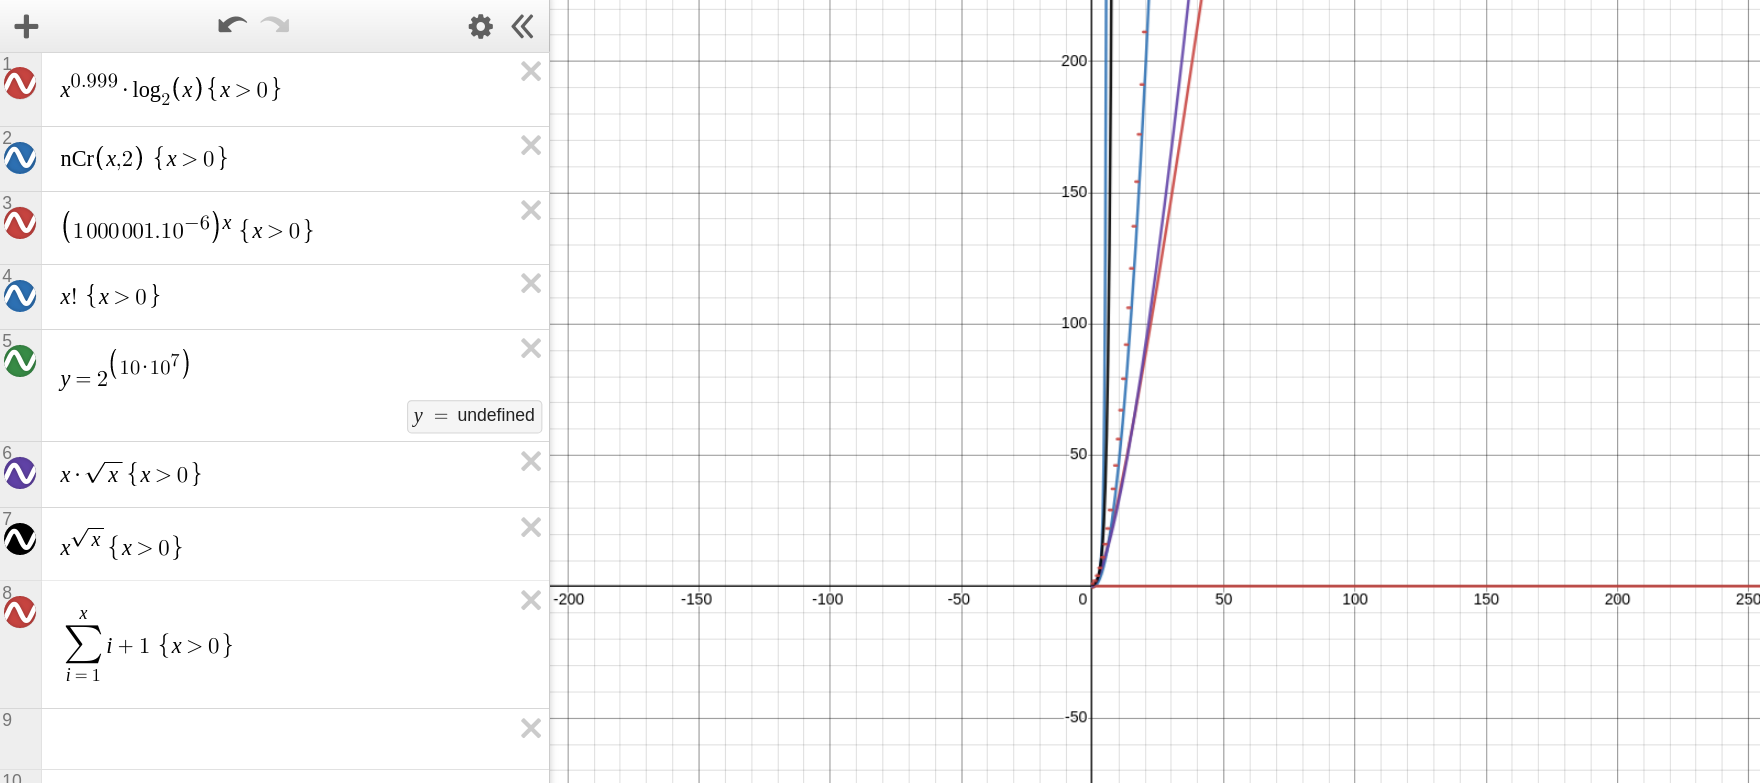
\includegraphics[width=1\linewidth]{image.png}
    \caption{Plotted Function in Desmos}
    \label{fig:enter-label}
\end{figure}
\\
N.B - $f_5$ is a large value ($2^{10^8}$) so it didn't fit inside the graph.
\subsection{Solution}
The complexities of the given equations are -
\begin{enumerate}
    \item $f_1(n) = n^{0.999}.\log_2(n)$
    \\
    For any c>0, $\log_2(n)$ is $O(n^c)$. \\So, $n^{0.999}.\log_2(n) = O(n^{0.999} . n^{0.001}) = O(n)$
    \\
    \textbf{Complexity} = $O(n)$ or linear
    \item $f_2(n) = \binom{n}{2}$
    \\
    $\binom{n}{2} = \frac{n(n-1)}{2} $
    \\
    \textbf{Complexity} = $O(n^2)$ or polynomial
    \item $f_3(n) = (1000001 * 10^{-6})^{n}$
    \\
    $(1000001 * 10^{-6})^{n} = 1.000001^{n}$
    \\
    \textbf{Complexity} = $O(1.000001^{n})$ or exponential
    \item $f_4(n) = n!$
    \\
    \textbf{Complexity} = $O(n!)$ or factorial
    \item $f_5(n) = 2^{(10*10^{7})}$
    \\
    \textbf{Complexity} = $O(1)$ or constant
    \item $f_6(n) = n*\sqrt{n}$ 
    \\
    \textbf{Complexity} = $O(n^{3/2})$ or polynomial
    \item $f_7(n) = n^{\sqrt{n}}$
    \\
    $n^{\sqrt{n}} = (2^{logn})^{\sqrt{n}} = 2^{\sqrt{n}logn} $
    \\
    \textbf{Complexity} = $O(2^{\sqrt{n}logn})$
    \item $f_8(n) = \sum_{i=1}^{n} (i+1)$ 
    \\
    $\sum_{i=1}^{n} (i+1) = \frac{n^2 + n}{2} + n = \frac{n^2 + 3n}{2}$
    \\
    \textbf{Complexity} = $O(n^2)$ or polynomial
\end{enumerate}
\newpage
\subsection{Complexity Comparison}
So, the increasing order of complexity --
\begin{center}
\begin{tabular}{|c|c|c|c|c|}
\hline
\multicolumn{5}{|c|}{Complexity Comparison} \\
\hline
\textbf{Rank} & \textbf{Function} & \textbf{Values} & \textbf{Complexity} & \textbf{$O(n)$} \\
\hline
1 & $f_5(n)$ & $2^{(10*10^{7})}$ & Constant & $O(1)$ \\
\hline
2 & $f_1(n)$ & $n^{0.999}.\log_2(n)$ & Linear & $O(n)$ \\
\hline
3 & $f_6(n)$ & $n*\sqrt{n}$ & Polynomial & $O(n^{1.5})$ \\
\hline
4 & $f_2(n)$ & $\binom{n}{2}$ & Polynomial & $O(n^2)$ \\
\hline
5 & $f_8(n)$ & $\sum_{i=1}^{n} (i+1)$ & Quadratic & $O(n^{2})$ \\
\hline
6 & $f_7(n)$ & $(n)^{\sqrt{n}}$ & Exponential & $O(2^{\sqrt{n}logn})$ \\
\hline
7 & $f_3(n)$ & $(1000001 * 10^{-6})^{n}$ & Exponential & $O(1.000001^{n})$ \\
\hline
8 & $f_4(n)$ & $n!$ & Factorial & $O(n!)$ \\


\hline
\end{tabular}
\end{center}
\vspace{5pt}

\newpage
\section{Task 2}
\subsection{Find only the complexity for find3RDelement function}

\begin{minted} [breaklines] {python}
def find3RDelement(a):
    flag = 2
    for i in range(len(a)):
        if i == flag : return a[i]
    print(find3RDelement([1,2,7,4,5]))
\end{minted}

The function \textbf{find3RDelement} searches for the 3rd element in a list. Whatever the length of the list is in the 3rd iteration the loop will return the the value. Thus the \textbf{find3RDelement} is constant or \textbf{O(1)}.


\newpage
\subsection{Find only the complexity for doingSomethingImportant}

\begin{minted} [breaklines] {python}
def doingSomethingImportant(p2,sr,sc,prev,new):
    row = len(p2)
    col = len(p2[0]) if len(p2) > 0 else 0
    if sr < 0 or sr >= row or sc < 0 or sc >= col :
        return
    if p2[sr][sc] != prev :
        return
    p2[sr][sc] = new
    doingSomethingImportant(p2 , sr - 1 , sc , prev , new)
    doingSomethingImportant(p2 , sr + 1 , sc , prev , new)
    doingSomethingImportant(p2 , sr , sc + 1 , prev , new)
    doingSomethingImportant(p2 , sr , sc - 1 , prev , new)

\end{minted}

The \textbf{doingSomethingImportant} function is a flood fill algorithm. The time complexity of the algorithm depends on the size of the array. Thus for an array with $n$ rows and $m$ columns, the complexity will be $O(nm)$.

\newpage
\subsection{Find only the complexity for doingSomethingImportant}
\begin{minted} [breaklines] {python}
def doingSomethingImportant(adj, V, sc):
    pq = [ ]
    heapq.heappush(pq,(0,sc))
    cost = [float('inf')] * V
    cost [sc] = 0
    while pq:
        d, u = heapq.heappop(pq)
        for v , weight in adj[u]:
            if cost[v] > cost[u] + weight:
                cost[v] = cost[u] + weight
                heapq.heappush(pq,(cost[v],v))
    return cost
\end{minted}
The \textbf{doingSomethingImportant} function is the Dijkstra algorithm to find the shortest path from one node to another. The implementation uses a priority queue/min-heap. Thus the complexity will be 
$O((V+E)\ log V)$.

\newpage
\section{Task 3}

\subsection{Solution}
\textbf{2D Peak - Binary Search (Recursive)}
\\
Steps:
\begin{enumerate}
    \item Pick middle column j = m/2
    \item Find global maximum on column j at (i, j)
    \item Compare (i, j − 1), (i, j), (i, j + 1)
    \item Pick left columns if (i, j − 1) > (i, j) , Otherwise pick right columns
    \item (i, j) is a 2D-peak if neither condition holds 
    \item Solve the new problem with half the number of columns.
    \item When you have a single column, find global maximum and you‘re done.
    
\end{enumerate}
Whenever the domain is reduced to a single column, the coordinate having the max value of that column is its 2D peak.
    
\subsection{Algorithm}
\begin{minted} [breaklines] {python}

def peakFinder2D_binary(matrix):
    
    rows, cols = matrix.shape

    if cols == 1:  # Base case
        return np.argmax(matrix[:, 0]), 0

    mid_col = cols // 2
    max_row_index = np.argmax(matrix[:, mid_col])
    max_val = matrix[max_row_index, mid_col]

    if mid_col > 0 and matrix[max_row_index, mid_col - 1] > max_val:
        # Recurse on left half
        return peakFinder2D_binary(matrix[:, :mid_col])  

    elif mid_col < cols - 1 and matrix[max_row_index, mid_col + 1] > max_val:
        # Recurse on right half
        return peakFinder2D_binary(matrix[:, mid_col + 1:])  
    
    else:
        return max_row_index, mid_col  # Found a peak
\end{minted}

\subsection{Complexity}
    \begin{itemize}
        \item \textbf{Divide-and-Conquer Approach :} The function recursively divides the matrix in half, effectively halving the search space in each iteration. This logarithmic behavior leads to the \textbf{log(m)} component in the complexity.
        \item \textbf{Finding Maximum in a Column:} The argmax operation used to find the maximum element in a column takes \textbf{O(n)} time, as it needs to iterate through all elements in that column. This contributes to the n component in the complexity.
        \item \textbf{Overall complexity :} Combining these two factors, we find the total complexity as \textbf{O($n*log_2(m)$)}
    \end{itemize}
    In every iteration we are reducing the search domain by half in terms of columns. So the 
\textbf{Complexity = O($n*log_2(m)$)} 
 where n and m is the number of row and columns respectively.

\end{document}
